% Chapter 3

\chapter{Analyzer Overview} % Main chapter title

\label{Chapter3}

\section{Theoretical Construction}
The development of our tool followed a structured, multi-step approach. As outlined in \capref{Chapter1}, to assess comment quality, it was necessary to categorize comments based on specific criteria, as illustrated in the figure below.

\begin{figure}[ht]
	\centering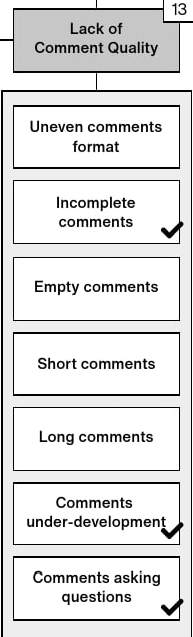
\includegraphics[height=350pt]{figs/goal-schema.PNG}
	\captionsetup{justification=centering}
	\caption{Comment categories the tool must be able to identify.}
	\label{fig:goal-schema}
\end{figure}

\noindent We began with simpler detections, such as identifying empty comments and comments that posed questions. Established rules were applied to determine if a comment was empty or contained either direct or implied questions.

\noindent Next, we tackled short and long comments. To achieve this, we utilized the \href{https://www.nltk.org/}{Natural Language Toolkit (NLTK)}, a comprehensive suite for natural language processing. By tokenizing each comment, we measured its length to classify it as either too short or overly long.

\noindent For comments under development, we employed pattern recognition techniques. We incorporated technical keywords and common phrases used during development to detect these comments.

\noindent The detection of incomplete comments and uneven comments format was refined through an iterative trial-and-error process, manually verifying results at each step. For incomplete comments, we initially performed a syntactic analysis to ensure the comments adhered to basic rules of English sentence structure. Subsequently, we built a classification system to categorize comments as single-line, multi-line, or documentation. For documentation comments, we verified consistency between the number of parameters in the comment and the corresponding source code, along with matching return types. Additionally, we introduced checks for single-line and multi-line comments to identify nonsensical or "gibberish" content, hence marking those that lacked clarity or coherence as incomplete.

\noindent Finally, for detecting uneven formatting, we flagged comments with irregular indentation, spacing, or annotation tag misuse, tailored to the programming language in use. This ensured that comments maintained proper structure, readability, and compliance with language-specific conventions.

\section{Logic Construction}

\begin{figure}[ht]
	\centering\includegraphics[width=400pt]{figs/whole-architecture.PNG}
	\captionsetup{justification=centering}
	\caption{General view on the tool's architecture.}
	\label{fig:whole-architecture}
\end{figure}

\noindent Let's discuss the architecture of our tool, which is organized into multiple layers. To provide clarity, we'll start with the foundational elements.

\begin{figure}[ht]
	\centering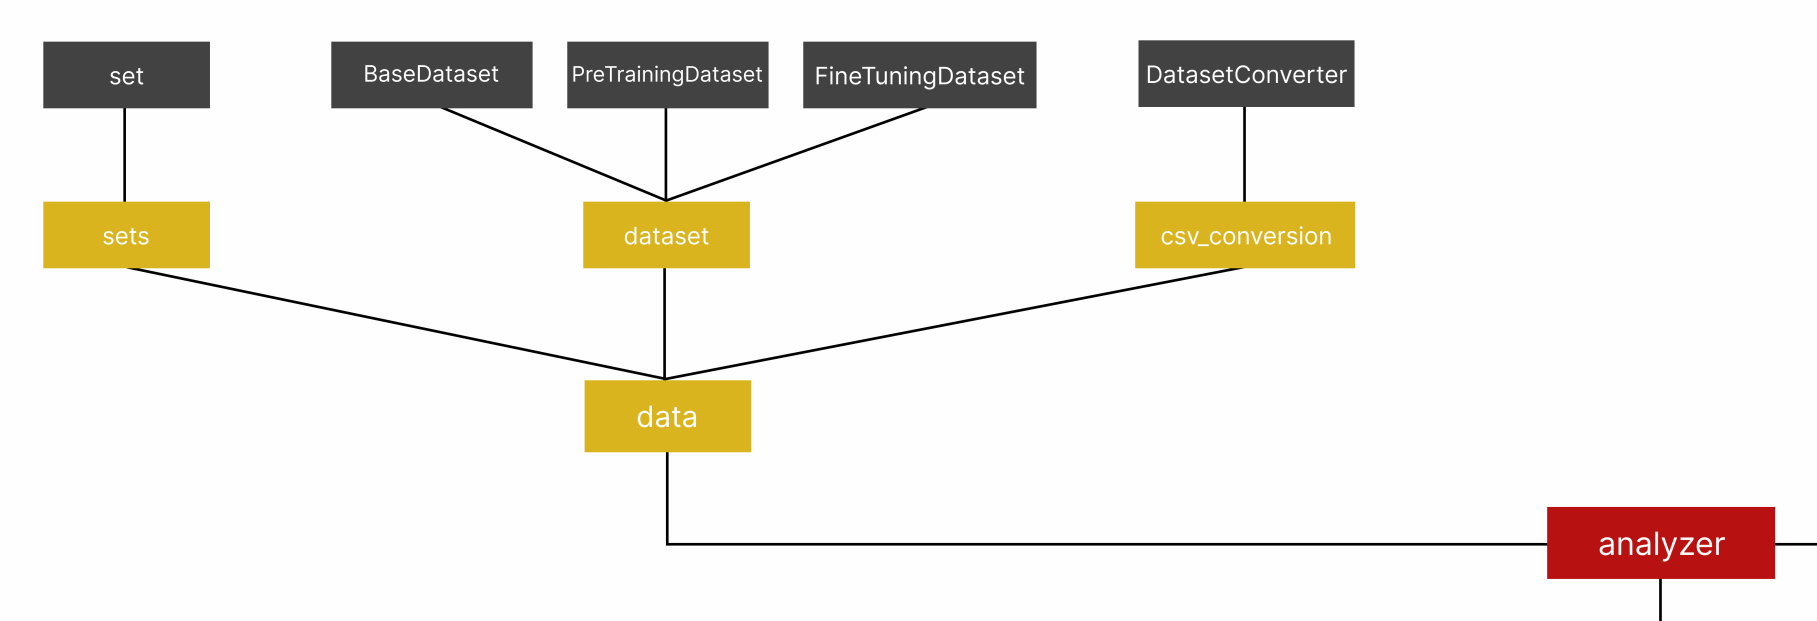
\includegraphics[width=400pt]{figs/zoom-data.PNG}
	\captionsetup{justification=centering}
	\caption{Zoom on the tool's data package.}
	\label{fig:zoom-data}
\end{figure}

\noindent The "data" package consists of three sub-packages:
	\begin{enumerate}
		\item \textbf{sets}: this sub-package contains the 'set' class, which defines the supported dataset file formats that our tool can read. The supported file extensions include \textit{.csv}, \textit{.tsv}, \textit{.json}, and \textit{.jsonl}.
		\item \textbf{dataset}: this sub-package contains several key classes:
			\begin{enumerate}
				\item \textbf{BaseDataset}: it provides a common interface for loading and working with various datasets, such as training, validation, and test sets.
				\item \textbf{PreTrainingDataset}: inheriting from BaseDataset, this class is designed to handle datasets specifically for pre-training models.
				\item \textbf{FineTuningDataset}: also inheriting from BaseDataset, this class is used for managing datasets in fine-tuning tasks.
			\end{enumerate}
		Both the \textit{PreTrainingDataset} and \textit{FineTuningDataset} classes default to the 'train' dataset if a specific set is not explicitly defined.
		\item \textbf{csv\_conversion}: this sub-package includes the \textit{DatasetConverter} class, which is used in cases where dataset format conversion is necessary.
	\end{enumerate}
	
\begin{figure}[ht]
	\centering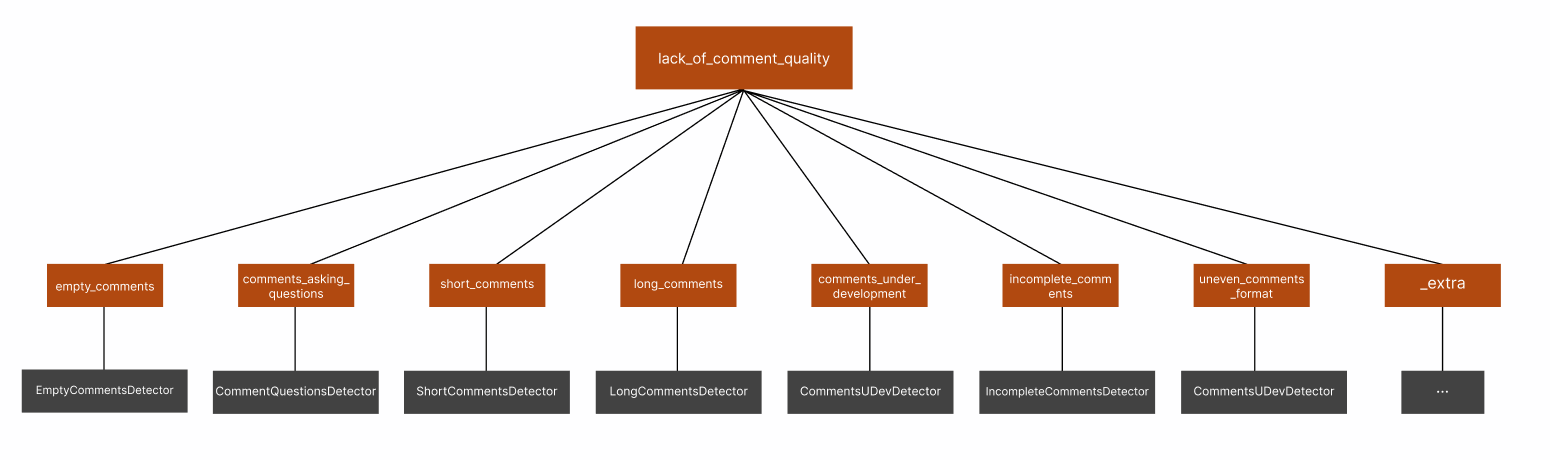
\includegraphics[width=465pt]{figs/zoom-cmsquality.PNG}
	\captionsetup{justification=centering}
	\caption{Zoom on lack of comments quality package.}
	\label{fig:zoom-cmsquality}
\end{figure}
	
\noindent The "smells" package contains our various detectors. I'm going to focus only on the "lack\_of\_comment\_quality" sub-package as the others are not part of this work.

\noindent Let’s begin with the "extra" sub-package, which might sound like an add-on, but contains essential components without which our tool wouldn't function.

\begin{figure}[ht]
	\centering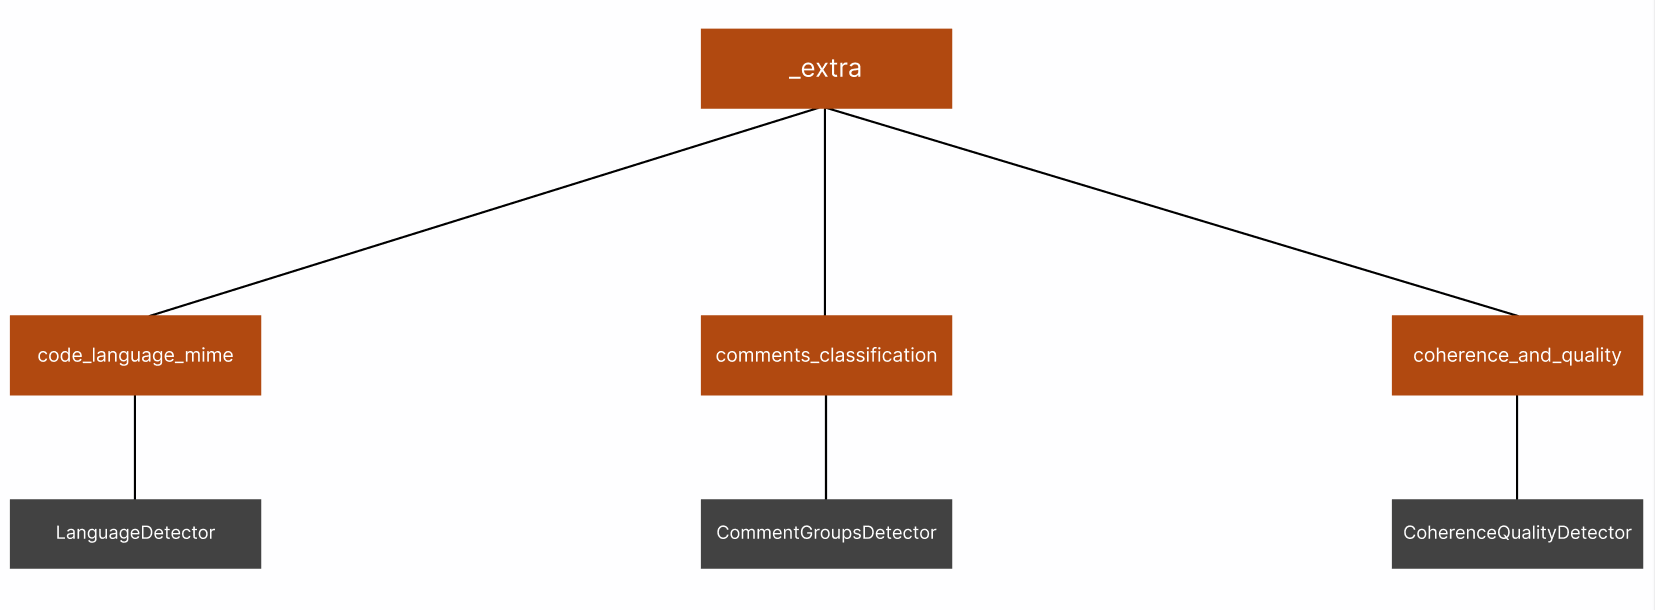
\includegraphics[width=400pt]{figs/zoom-extra.PNG}
	\captionsetup{justification=centering}
	\caption{Zoom on extra sub-package.}
	\label{fig:zoom-extra}
\end{figure}

\noindent Initially, we aimed for the tool to be language-agnostic, meaning it would work with all programming languages. While this is true for some detectors, it’s not feasible for all. As a result, we introduced a programming language detector, represented by the "code\_language\_mime" sub-package and its corresponding \textit{LanguageDetector} class. This class uses the \href{https://github.com/jossef/guesslang}{guesslang} library to identify the programming language used in a dataset and maps it to its MIME type.

\noindent The \textit{CommentGroupsDetector} class, located in the "comments\_classification" sub-package, scans all comments in the input database and categorizes them as single-line, multi-line, or documentation comments. This classification is crucial for enabling the incomplete comments detector and the uneven comments format detector to function correctly.

\noindent An additional detector, the \textit{CoherenceQualityDetector}, resides in the 

\noindent "coherence\_and\_quality" sub-package. This detector was developed while researching comment completeness, but it doesn’t strictly relate to incomplete comments, so it was placed in a separate package. The detector evaluates comments based on the following criteria:
	\begin{itemize}
		\item \textbf{Language (L)}: Ensures the comment is not written in a mix of different languages.
		\item \textbf{Clarity (C)}: Uses NLP techniques to assess the readability of the comment.
		\item \textbf{Relevance (R)}: Verifies that the comment accurately describes the specific code constructs it’s meant to explain.
		\item \textbf{Brevity (B)}: Checks if the comment avoids unnecessary repetition or wordiness.
		\item \textbf{Context (X)}: Determines whether the comment provides sufficient explanation for understanding the code.
	\end{itemize}
If a comment meets all these criteria, it is considered coherent. Otherwise, it is flagged as incoherent.

\noindent Let me now explain the "examples" package before listing the heuristics for the main smell detectors in the next paragraph.

\begin{figure}[ht]
	\centering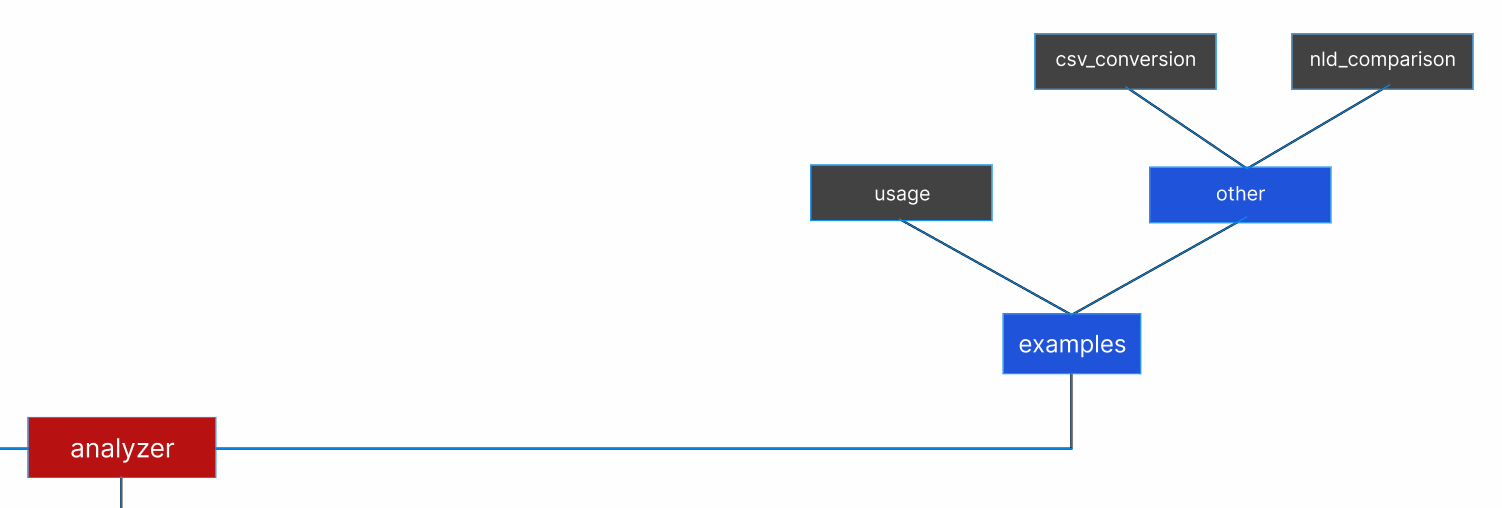
\includegraphics[width=400pt]{figs/zoom-examples.PNG}
	\captionsetup{justification=centering}
	\caption{Zoom on examples sub-package.}
	\label{fig:zoom-examples}
\end{figure}

\noindent The "examples" package contains the execution scripts for our tool. The key script is "example\_usage", which serves as the main file. This script loads the input dataset and sample, runs the desired detectors, and collects the results, returning a complete list of findings once the analysis is finished.

\noindent Within the "other" sub-package, there are two additional scripts:
	\begin{itemize}
		\item \textbf{example\_csv\_conversion}: this script uses the similarly named sub-package in "data" to convert raw datasets into a more readable format for the tool.
		\item \textbf{example\_nld\_comparison}: this script stems from a detailed study comparing the speed and accuracy of two NLP libraries, \href{https://spacy.io/}{\textit{spaCy}} and \href{https://fasttext.cc/}{\textit{fastText}}, for natural language detection. In our tool, language detection is essential for incomplete comment detection, as we first check whether a sentence is written in English. To evaluate the two libraries, we created a dictionary with words from eight different languages, then shuffled and combined them to generate a sample of 3,000 groups of sentences, where each is written in a different language. Both libraries successfully detected all languages, but spaCy took 99.51 seconds to complete, while fastText only required 24.25 seconds. Given its significantly superior speed, we opted for fastText for natural language detection in our tool.
	\end{itemize}